\section{Esoteric Darwinism}

I spent a few hours this week reading some reviews of \emph{Mind and Cosmos} by \textbf{Thomas Nagel}; I
hadn't realized it was such a widely reviewed work. There are some broad categories of reviews. After
briefly describing them, I will offer the esoteric interpretation. Finally, we will explain why Zarathustra was so
frustrated.

\paragraph{Materialism}
\begin{wrapfigure}{rt}{.35\textwidth}
 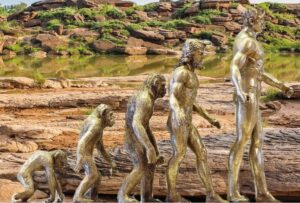
\includegraphics[scale=.5]{a20151116EsotericDarwinism-img001.jpg} 
\end{wrapfigure}

There are the diehard materialists who reject the argument \emph{a priori}. The objection is to the introduction of
“mysterious” forces like mind, teleology, and so on. I suppose that familiarity breeds contempt, since gravity,
electromagnetism, quantum mechanics, the big bang, the origin of life, etc., are themselves quite mysterious. Moreover,
the claim that “matter” follows “laws” is itself an indication that there is intelligence inherent in matter. On the
other hand, consistent positivists like Stephen Hawking admit that scientific theories have merely pragmatic value, but
tell us nothing about ultimate reality.

Ultimately, there is no way to resolve the conflict between materialism and idealism in thought alone. What the latter
finds intelligible, the former considers just a serendipitous sequence embedded in a purely random sequence. It seems,
also, that it is impossible for real materialists to consider subjective conscious experiences of any significance. It
really comes down to differences in people and how they experience inner states. Some just don't seem to
have a very vivid interior life.

\paragraph{Sympathetic Views}
There are broadly sympathetic views. However, they don't seem to share Nagel's viewpoint;
rather, they latch onto the criticisms of neo-Darwinism. Nagel himself describes his point of view this way:

\begin{quotex}
The view that rational intelligibility is at the root of the natural order makes me, in a broad sense, an
idealist —not a subjective idealist, since it doesn't amount to the claim that all reality is
ultimately appearance— but an objective idealist in the tradition of Plato and perhaps also of certain
post-Kantians, such as Schelling and Hegel, who are usually called absolute idealists. 

\end{quotex}
I couldn't find a review by an “absolute idealist”; perhaps there aren't any left. Nagel claims
that absolute idealism was simply abandoned, not refuted.

Curiously, a Thomist thinker wrote that Nagel's view is an “essentially neo-Aristotelian position”. It would
be interesting, but also welcome, to classify neo-Aristotelians among the absolute idealists. The idealists
I've read would certainly have benefited by the inclusion of Aristotelean elements, in particular,
hylomorphism. Certainly, Julius Evola did so with great effect with his ideas about essence, existence, and privation.
For Rene Guenon, too, the notion of the Absolute was fundamental. Certainly, he combined ideas from the Samkhya school
(purusha/prakriti) within his Vedantic approach.

Absolute idealism starts from “above”; i.e., it begins with the notion of the Absolute and derives the world.
Aristotelianism starts from “below”, with sense experience, and by analogy reaches the Absolute.

\paragraph{Neotheism}
There is a view called Neotheism, which considers God as a very powerful being among other beings, rather than as the
Absolute or Being itself. Actually, this is the idea of God in the popular mind, rather than the true classical idea.
Even atheists, for the most part, refute such a neo-god, thereby missing the point. If such a being exists, then there
is still the Absolute – rather confusing.

Although this group likes Nagel's critique of neo-Darwinism, it is really not very helpful. In effect, this
view is not unlike the naïve realism of the materialists: the world is out there, right now, in some spatial container
in time. However, they then presume that the neo-god provides the goal and meaning to this space-time material world.
The world in itself is meaningless, just as it is for the materialists. They add to this world invisible beings and
miracles that seem to come from nowhere.

\paragraph{Mystical Evolution}
It seems, then, that we are faced with an impossible dilemma: accept science or accept a spiritual life. On the other
hand, \textbf{Valentin Tomberg} gave us the teaching of Practical Monism, which reconciles, or neutralizes, the pair of
opposites. However, that is accomplished not in the realm of speculative thought but rather in practical reason. That
is, it is only by living, not just by thinking, that the dualism in thought is resolved in a practical monism.

The materialist view is consistent with esoteric teaching. For example, \textbf{Boris Mouravieff} writes this in
\emph{Gnosis}, Vol 1:

\begin{quotex}
Properly speaking, this kind of existence cannot be considered as human; it could be described as anthropoid. This term
is justified in the sense that exterior man, immersed in self-satisfaction, represents the crowning achievement of
millions of years of evolution of the species from its animal ancestors, yet, from the point of view of esoteric
evolution, he is a possibility which has not yet been realized. 

\end{quotex}
So the scientific teaching that man, as he is, is an ape, an anthropoid, is consistent with esoteric teaching. Like all
animal life, the anthropoid man is under the dominance of the General Law of fear, sex, and hunger. All his ideals are
illusory epiphenomena, supervening on a bed of genetic, libidinal (Freud), and economic (Marx) forces.

That is the first birth. The initiation into the true life of the spirit is the second birth; the anthropoid gives birth
to the man as he should be. He seeks to overcome the general law of biological life in order to realize his True Self.
This is not an automatic or material process. Rather, it must be freely chosen and it requires conscious efforts. In
other words, he becomes his aim in life.

\paragraph{Zarathustra}
\begin{quotex}
Transformed is Zarathustra; Zarathustra has become a child; an awakened one is Zarathustra: what will you do in the land
of the sleepers?

I love him who lives in order to know, and seeks to know in order that the overman may someday live. \flright{\textsc{Friedrich Nietzsche}, \emph{Thus Spoke Zarathustra}}

\end{quotex}
Just as in the case of Galileo, people have heard rumors about Darwin, but its meaning has not yet sunk in. For the
educated it is important to “believe in evolution”. But to believe that, is also to believe you are an anthropoid. Yet
the modern man believes that he is the goal of evolution, its acme, and that nothing could be conceivably be higher.
Thus he is the last man and proud of it. If everyone would be just like him, the Kingdom would arrive and the evil ones
would be transported away on a cloud. There would be no war, no global warming, and so on.

So Zarathustra told them they were anthropoids, since they should want to know. Instead, they banished him, because in
the Country of the Blind, the seer is a menace.

\flright{\itshape Posted on 2015-11-16 by Cologero}
